\mysection{1}{Generalities and Map Reduce}
I problemi "big data" fanno riferimento a quella tipologia di problemi dove il carico dei dati da elaborare è MOLTO grande. Per risolvere un problema di questo tipo, una volta, avremmo fatto affidamento su un unico "super computer". Oggi, si utilizzano strutture di più dispositivi uniti chiamate \textbf{computer clusters}.
\\
\begin{figure}[th]
    \centering
    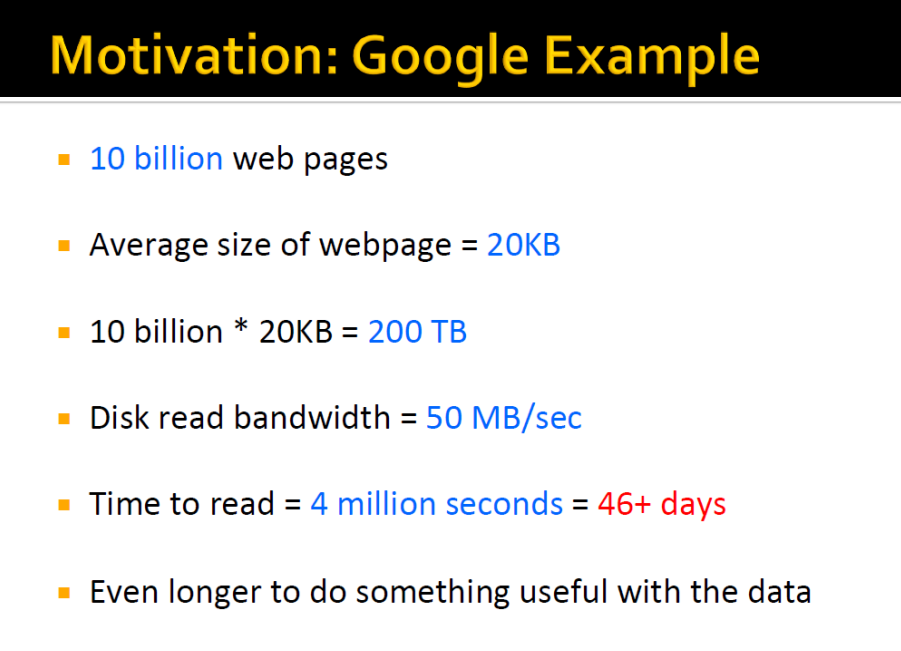
\includegraphics[scale=0.35]{MapReduce/img/GoogleExample.png}
    \label{fig:googleex}
\end{figure}
\\
L'esempio principale lo abbiamo da Google: elaborare dati con poche macchine sarebbe infattibile. Quello che faremo sarà quindi andare a mettere insieme più server ma la loro gestione rimane un problema grande. Cosa succede se ho bisogno di un'informazione ma si rompe una macchina che permetteva di accedervi? 
\subsection{Introduction to Distributed File Systems}
Consiste nello store dei dati in maniera \textit{redundant}: ovvero frammentando l'informazione in più chunks per potervi risalire in qualunque momento. In questo modo riesco ad avere più copie approssimative della mia informazione sparse per la mia rete. La dimensione dei chunk e il grado di riproduzione del dato sono decisi dall'utente. 
\\
\textit{Come gestisco i chunk?} Il \textbf{Master node} è il contenitore del filesystem tree, delle metadata e le directories. Attraverso esso gestiamo i chunks. Anche il master node viene replicato. 
\\
Ma quindi, come elaboro i dati nel Distributed File System? Con il metodo \textbf{Map Reduce}.
\newpage

\subsection{Map Reduce}
Ci permette di leggere sequenzialmente grandi quantità di dati. Si compone principalmente di tre step:
\begin{enumerate}
    \item Map
    \item Group by key
    \item Reduce
\end{enumerate}
\textbf{\large{map}}
\\[2ex]
Il "map" è il primo step dove essenzialmente vado alla ricerca delle informazioni utili. Corrisponde di fatto ad una query dove isolo elementi secondo una certa caratteristica. \textit{Extracting something of interest}
\\[2ex]
\textbf{\large{group by key}}
\\[2ex]
Fare "group by key" significa letteralmente "raggruppare per chiave". Aggrego cose simili tra di loro, ma tengo il conto di quante ne ho raggruppate. Di fatto, metto insieme la chiave e tutti i valori a lei associati. 
\textit{Sort and shuffle}
\\[2ex]
\textbf{\large{reduce}}
\\[2ex]
Mette insieme tutto alla fine, aggrega per avere dei dati più compatti. Risparmiando quindi memoria semplicemente associando, ad ogni elemento diverso del documento, il numero di volte che si ripete.
\textit{Aggregate, summarize, filter, transform}
\\
\begin{figure}[th]
    \centering
    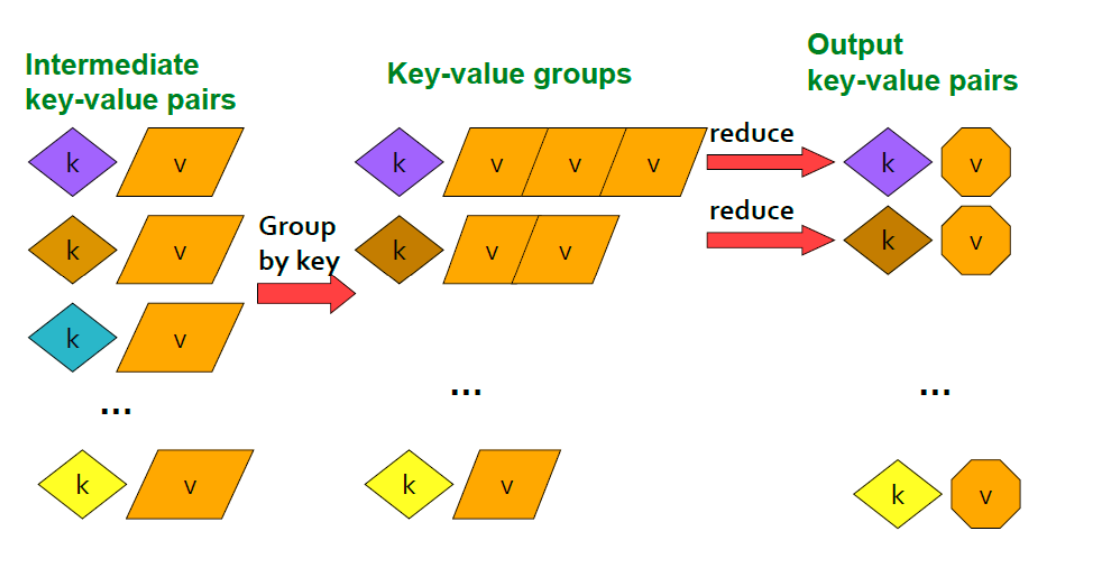
\includegraphics[scale=0.5]{MapReduce/img/MapReduce.png}
    \label{fig:mapreduce}
\end{figure}
\\
Piccolo approfondimento per pura curiosità: è nato per risolvere il problema della ricerca e conteggio di parole per Google. 

\newpage

\subsection{Distributed File System Architecture w/ Map Reduce}

Possiamo immaginare il Master Node come colui che gestisce gli altri nodi, identifica le operazioni che gli altri devono compiere. Ad esempio, nella ricerca e conteggio delle parole, una parola che si ripete lui la invia a chi di dovere per farla ridurre, ovvero identifica un gruppo di nodi adibiti a questa funzione. Nell'immagine seguente è possibile notare tutti i pezzi di un Distributed File System e la loro funzione. 
\\
\begin{figure}[th]
    \centering
    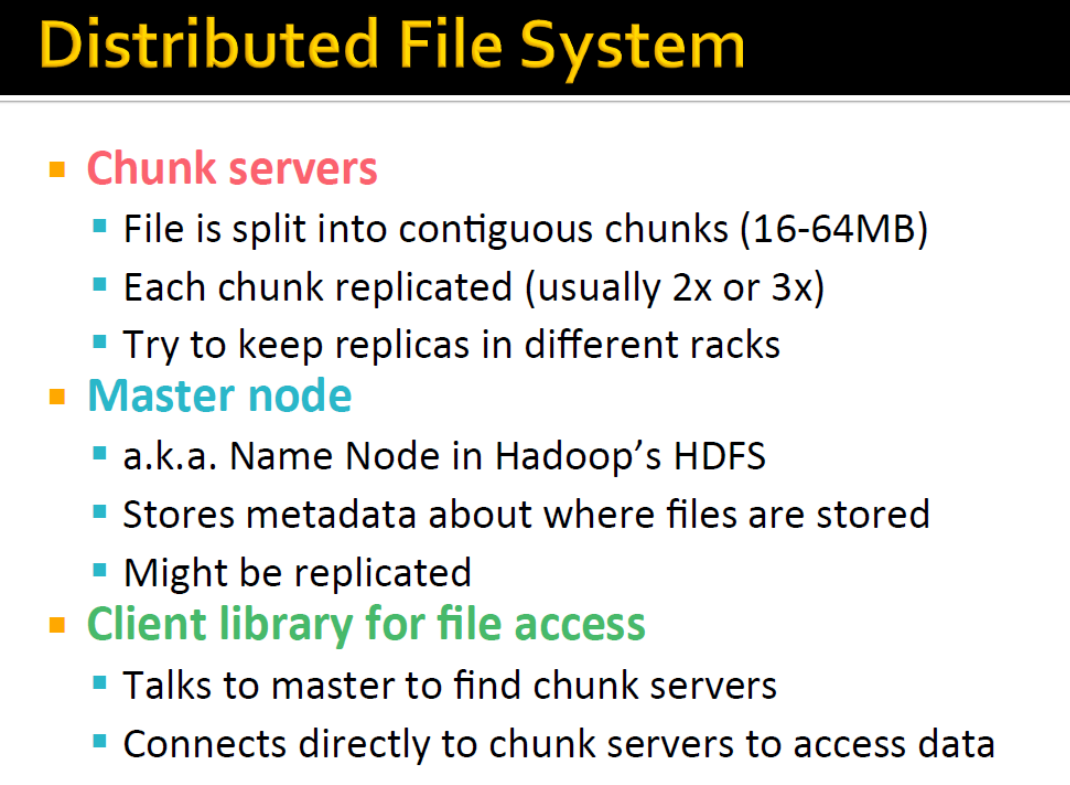
\includegraphics[scale=0.4]{MapReduce/img/DFS.png}
    \label{fig:DFS}
\end{figure}
\\
Inoltre, il Master Node controlla e pinga periodicamente i workers per trovare delle failures (malfunzionamenti).
\\
\textbf{Cosa succede se avviene un guasto?} Dipende da che parte della struttura si rompe:
\begin{itemize}
    \item Map worker: le task del worker sono resettate, i reduce workers vengono notificati quando la task viene compiuta da un altro worker
    \item Reduce worker: solo le task in-process del worker vengono resettate, la task di reduce viene restartata
    \item Master failure: MapReduce task abortita e contattato il client
\end{itemize}
La funzione di Reduce è associativa e commutativa, quindi va utilizzati in casi compatibili ad essa: se devo contare o sommare, posso utilizzarla. Ad esempio invece se dovessi fare la media mi sarebbe impossibile farlo! 
\\
I valori possono essere combinati a piacimento che danno lo stesso risultato. I valori delle key/value di input devono essere dello stesso tipo dei valori delle key/output. (Commutativa e Associativa)
\newpage
\subsection{MapReduce in parallelo}
Vengono mappati più valori e viene eseguita la reduce su più dati separati secondo un determinato criterio: 
\begin{figure}[th]
    \centering
    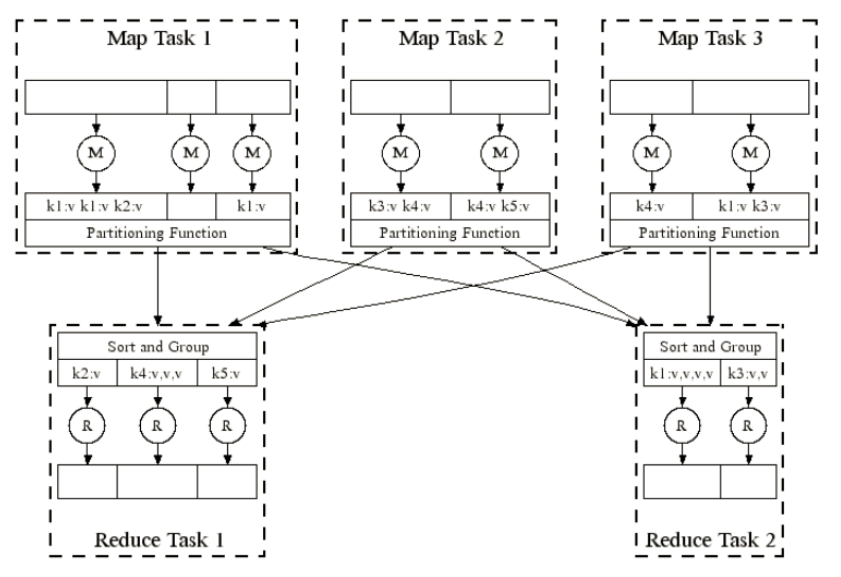
\includegraphics[scale=0.5]{MapReduce/img/MapReduceParallel.png}
    \label{fig:mapreduceparallel}
\end{figure}

\subsection{Combiners}
I combiners sono elementi che ci aiutano a combinare il valore di tutte le chiavi di un singolo mapper (un singolo nodo) così non è necessario copiare e mescolare tutti questi dati. 
\begin{figure}[th]
    \centering
    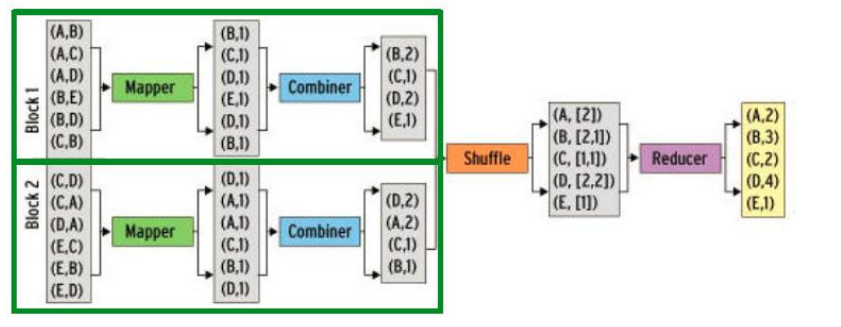
\includegraphics[scale=0.5]{MapReduce/img/Combiners.png}
    \label{fig:combiners}
\end{figure}

\subsection{Remarks}
Per raggiungere il massimo parallelismo, potremmo usare un Reduce Task per eseguire ogni reducer oppure eseguire ogni Reduce task in un nodo diverso. Ma tutte queste ipotesi genererebbero solo dei problemi in più: 
\begin{itemize}
    \item potrebbero esserci più chiavi dei nodi che abbiamo. 
    \item potrebbe esserci una variazione eccessiva della lunghezza delle liste di valori per chiavi diverse
    \item c'è un overhead associato ad ogni task che creiamo 
\end{itemize}

\subsection{Algoritmi che usano Map Reduce}
\textit{Elevata probabilità di essere chiesto.} Esistono diversi algoritmi che sfruttano il map reduce, come la moltiplicazione vettoriale oppure le operazioni di algebra relazionale. 

\subsubsection{Matrix-Vector multiplication - Vettore che sta in memoria}
Matrice M = n $\times$ n ($m_{ij}$), v = vettore di n componenti. Il prodotto matrice vettore fornisce come risultato:
\begin{center}
    \begin{math}
        x_i = \sum^{n}_{j=1} m_{ij} v_j
    \end{math}
\end{center}
M e v sono salvati entrambi nel DFS (Distributed File System) come coppie (i,j, $m_{ij}$) e (j, $v_j$). Per fare il map consideriamo sempre che v stia fisicamente in memoria. Ogni Map Task opera su un chunk di M. Per ogni $m_{ij}$ che legge, genera un (i, $m_{ij} v_j$), che banalmente è la moltiplicazione del valore ij-esimo della matrice per il valore j-esimo del vettore, e gli associa un altro indice i $\rightarrow$ la Reduce Task invece somma tutti i valori associati alla stessa key i, ottenendo (i, $x_i$). Si può vedere perfettamente questo passaggio dalle slide del professore: 
\\
\begin{figure}[th]
    \centering
    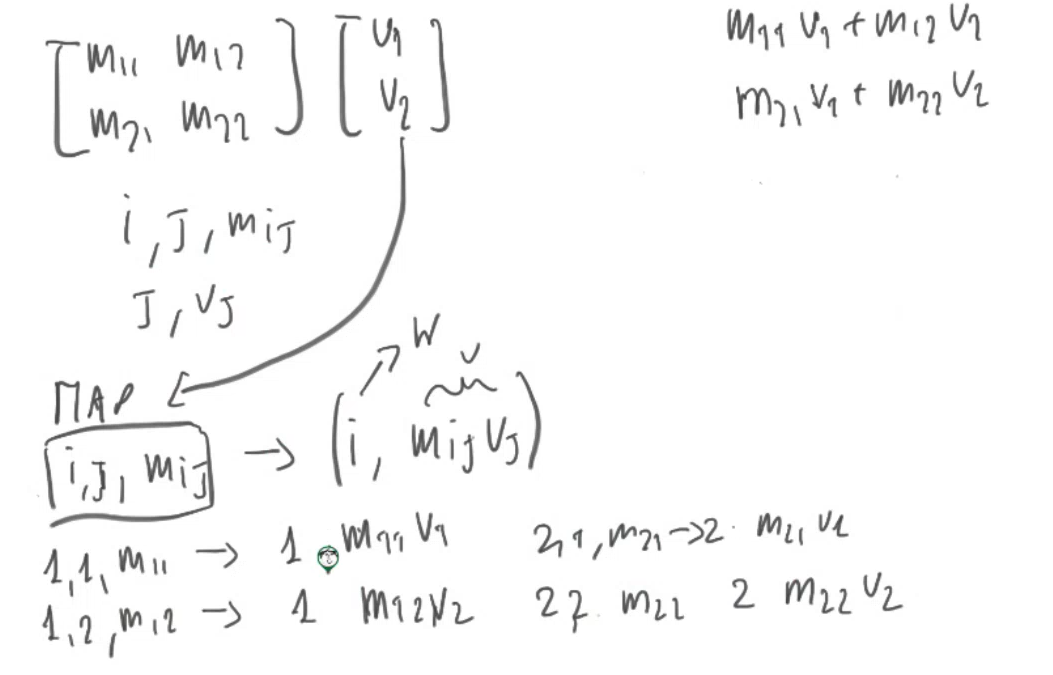
\includegraphics[scale=0.5]{MapReduce/img/MatrixVector.png}
    \label{fig:matrixvec}
\end{figure}
\\
Ora abbiamo il Group By Key Task, che funziona esattamente come spiegato: mette insieme gli elementi che hanno stessa chiave. La chiave, in questo caso, è la \textbf{riga della matrice}. Quindi, dopo la Reduce Task che fa la somma e osservando sempre l'immagine, il risultato che otterremo sarà:
\begin{center}
    \begin{math}
        [1, m_{11} v_1 + m_{12} v_2], [2, m_{21} v_1 + m_{22} v_2] 
    \end{math}
\end{center}
Che è esattamente il risultato dell'operazione matrice per vettore.

\newpage

\subsubsection{Matrix-Vector multiplication - Vettore che non sta in memoria}
Con v che non sta in memoria, semplicemente separiamo gli elementi di v in modo da ottenerne una quantità fattibile per la memoria. La cosa importante è che la parte della matrice che sarebbe da moltiplicare per quegli elementi, venga associata correttamente. Quindi dividiamo il vettore e la matrice in bande, e le associamo l'un l'altra, ottenendo una struttura ben associata e definita. 
\\
\begin{figure}[th]
    \centering
    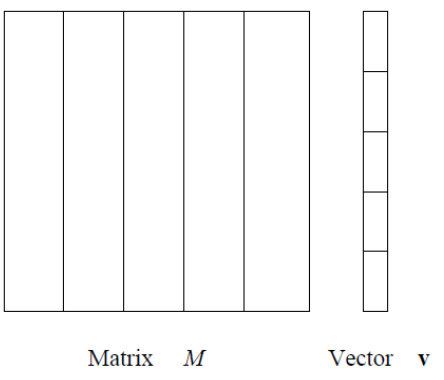
\includegraphics[scale=0.5]{MapReduce/img/MatrixSep.png}
    \label{fig:matrixmult}
\end{figure}

\subsubsection{Relational algebra operations - Selection}

$\sigma_C(R)$ 
\\
Mapping $\rightarrow$ per ogni tupla t che soddisfa C, emetti (t, t)
\\
Reducing $\rightarrow$ emette l'identità. NON fa altre operazioni.

\subsubsection{Relational algebra operations - Projection}

$\pi_S(R)$ 
\\
Mapping $\rightarrow$ per ogni tupla t costruisci t' rimuovendo i componenti i cui attributi non sono in S emetti (t', t'). 
\\
Reducing $\rightarrow$ emetti i key value pairs (t', t') rimuovendo i duplicati. 

\subsubsection{Relational algebra operations - Union}

$UNION(R, S)$ 
\\
Mapping $\rightarrow$ per ogni tupla t in input, emetti (t, t)
\\
Reducing $\rightarrow$ emetti (t,t). Associati alla chiave ci sono uno o due valori. L'unione di fatto elimina i duplicati.

\subsubsection{Relational algebra operations - Intersection}

$INTERSECTION(R,S)$ 
\\
Mapping $\rightarrow$ per ogni tupla t in input, emetti (t, t)
\\
Reducing $\rightarrow$ emetti (t,t) solo se ci sono 2 valori uguali (se le tabelle quindi si intersecano nella tupla). 

\subsubsection{Relational algebra operations - Difference}

$DIFFERENCE(R-S)$ 
\\
Mapping $\rightarrow$ per ogni tupla t di R in input, emetti (t, R) e per ogni tupla t in S emetti (t, S)
\\
Reducing $\rightarrow$ Per ogni key t, se la lista dei valori associati è R emetti (t) altrimenti nulla.

\subsubsection{Relational algebra operations - Natural Join}

$R(a,b) JOIN S(b,c)$ 
\\
Mapping $\rightarrow$ per ogni tupla (a,b) in R emetti (b,(a,R)) e per ogni tupla (b,c) in S emetti (b, (c,S)) 
\\
Reducing $\rightarrow$ Ogni key value b è associato a una lista di coppie (a,R) e (c,S) da cui puoi costruire tutte le coppie prendendo un elemento da R e uno da S. 

\subsubsection{Relational algebra operations - Grouping and Aggregation}

R(A,B,C) $\gamma_{A, \theta(B)}$(R) 
\\
Mapping $\rightarrow$ per ogni tupla (a,b,c) produce il key value (a,b)
\\
Reducing $\rightarrow$ applica l'aggregazione $\theta$ alla lista [b1,b2,...,bn] associata ad a; il risultato è una coppia (a,x) dove c è il risultato dell'aggregazione $\theta$. 
\\
Se ci sono attributi di aggregazione multipli il key value della map function è la lista dei valori e la reduce si applica ad ognuno di essi. 
\subsubsection{Matrix multiplication}
Il risultato di una moltiplicazione matriciale date due matrici \textit{m} e \textit{n} di dimensione $r_m \times c_m$ e $r_n \times c_n$ è una matrice $r_m \times c_n$, i cui valori:
\begin{center}
    \begin{math}
        p_{ik} = \sum_j m_{ij} n_{jk}
    \end{math}
\end{center}
\begin{figure}[th]
    \centering
    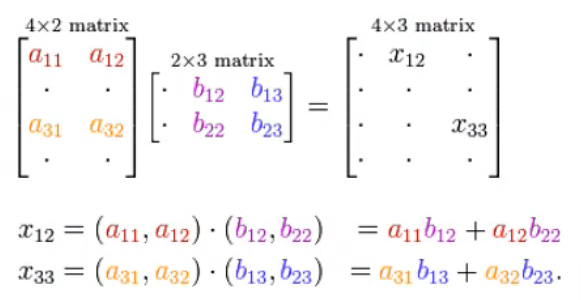
\includegraphics[scale=0.6]{MapReduce/img/MatrixMolt.png}
    \label{fig:matrixmolt}
\end{figure}
\textbf{Come viene risolta con Map Reduce?} Viene svolta con due Map Reduce in cascata. Nella Map Task prendiamo ogni elemento della matrice \textit{m} e \textit{n} e genero delle coppie chiave valore:
\begin{center}
    \begin{math}
        (j, (M, i, m_{ij})), (j, (N, k, n_{jk}))
    \end{math}
\end{center}
Dove M e N sono i nomi delle tue matrici. Ora nella Group by key Task andremo ad associare gli elementi con stessa chiave, producendo un elemento con chiave $(i,k)$ e valore $(m_{ij}n_{jk})$ e nella Reduce Task, faremo la somma. 
\newpage
\subsection{Remarks}
Per raggiungere il parallelismo massimo, possiamo: usare una Reduce task per eseguire tutti i reducer, oppure svolgere tutte le Reduce task ad un computer node diverso. Ma non è una linea guida ottimale, perchè ad esempio potremmo ottenere più keys dei compute nodes disponibili. Ulteriore problema è dato nell'esecuzione delle Reduce Tasks separate, che va ad aumentare il tempo di ogni operazione. 
\\
Per guardare il \textbf{costo} del Map Reduce, devo guardare il quantitativo dei dati, perchè l'operazione più costosa è il trasferimento di essi. A questo punto una soluzione sicuramente potrebbe essere quella di tenere una sola macchina (rimuovendo il parallelismo) necessitando così di una macchina sola che contenga tutti i miei dati. 
\\
\textbf{Dobbiamo bilanciare queste due cose.} Lo facciamo basandoci su due parametri, la \textbf{Reducer size} (che indichiamo con \textit{q}) e il \textbf{Replication rate} (che indichiamo con \textit{r}).
\subsubsection{Reducer size $q$}
Questo parametro indica il numero di valori associabili ad una key. Nell'architettura Combiner, questo valore è fisso a 1.
\subsubsection{Replication rate $r$}
Questo parametro indica il numero di coppie key-value che la lettura di un input mi genera. Esiste un algoritmo (non trattato a lezione) che è quello della moltiplicazione matriciale in uno step solo, che ha come $r$ il numero $k$ delle colonne quindi ad ogni input genero $k$ coppie. Ma di base lo abbiamo sempre considerato 1. 
\\[2ex]
\textbf{\large{Relazione tra $r$ e $q$}}
\\[2ex]
Sono inversamente proporzionali. Non si è espresso più di tanto riguardo a questi due valori perchè basta semplicemente sapere che giocando sulla loro proporzionalità è il modo giusto per bilanciare il costo delle operazioni. 
\subsubsection{Similarity Join}
\textit{Argomento importante.} L'esempio classico che lui utilizza per spiegare questo argomento, è un ds con $10^6$ immagini dove vogliamo cercare delle similitudini. Se utilizzassimo Map Reduce e applicassimo la Map Task ad un input (1, $I_1$), mettendolo in relazione con la generica immagine (j, $I_j$), otterremmo una coppia di questo tipo (i,j)($I_i ,I_j$) il che vorrebbe dire ottenere per ogni immagine, 999'999 valori. Replication rate $r$ elevatissimo, moltiplicato per 1 MB di immagine, e per ogni immagine presente (perchè il ragionamento è da iterare su tutte) otteniamo:
\begin{center}
    \begin{math}
        999'999 \times 10^8 \times 10^6 = 10^{18}
    \end{math}
\end{center}
Che sono EB. Con una rete Gbit, $10^8$ bit/s, ci vogliono 300 anni. L'approccio migliore da usare è quello della similarity join per cui separo il dataset in gruppi. Ottengo un $r$ = g - 1 (g è il numero di gruppi) quindi più gruppi faccio, più riduco il costo delle operazioni. Devo sempre tenere conto però che riducendo $r$, $q$ aumenta. La $q$ infatti diventa $\frac{n}{g}$ ovvero il numero di dati diviso il numero di gruppi, che indica il valore massimo che può assumere una chiave (se fosse simile a tutte le immagini del suo gruppo).